\documentclass[12pt,a4paper]{article}
\usepackage[UTF8]{ctex}
\usepackage{amsmath}
\usepackage{amssymb}
\usepackage{amsthm}
\usepackage{graphicx}
\usepackage{hyperref}
\usepackage{geometry}
\usepackage{algorithm}
\usepackage{algorithmic}
\usepackage{listings}
\usepackage{xcolor}
\usepackage{fancyhdr}
\usepackage{tikz}
\usetikzlibrary{arrows,positioning,calc}
\usepackage{pgfplots}
\pgfplotsset{compat=1.18}
\geometry{left=2cm,right=2cm,top=2.5cm,bottom=2.5cm,headheight=15pt}
\setlength{\baselineskip}{1.1\baselineskip}
\setlength{\parskip}{0.5em}

% 导入通用样式
% 通用样式文件 - 统一所有文档的样式

% 目录样式设置 - 干净简洁,无边框,优化编号
% 使用基本 LaTeX 命令美化目录
\makeatletter
\renewcommand\@dotsep{2}
% 优化编号格式:减少缩进,使编号更紧凑
\renewcommand\l@section{\@dottedtocline{1}{0em}{1.2em}}
\renewcommand\l@subsection{\@dottedtocline{2}{1.2em}{1.8em}}
\renewcommand\l@subsubsection{\@dottedtocline{3}{3em}{2.2em}}
% 设置目录深度为3,显示到subsubsection级别
\setcounter{tocdepth}{3}
\makeatother

% 超链接设置 - 目录链接无颜色框
\hypersetup{
    colorlinks=true,
    linkcolor=black,          % 目录链接为黑色
    filecolor=black,
    urlcolor=blue,
    citecolor=black,
    pdfstartview=FitH,
    pdfborder={0 0 0},        % 无边框
    linkbordercolor={0 0 0},  % 链接边框颜色为黑色(不可见)
    pdfborderstyle={/S/U},    % 无边框样式
}

% 页眉页脚设置(在文档中重新定义)
\usepackage{fancyhdr}
% 注意:每个文档需要在导入 common_style.tex 后设置自己的页眉页脚

% 章节格式 - 简洁美观(使用基本命令)
\makeatletter
\renewcommand\section{\@startsection {section}{1}{\z@}%
                                   {-3.5ex \@plus -1ex \@minus -.2ex}%
                                   {2.3ex \@plus.2ex}%
                                   {\normalfont\Large\bfseries}}
\renewcommand\subsection{\@startsection{subsection}{2}{\z@}%
                                     {-3.25ex\@plus -1ex \@minus -.2ex}%
                                     {1.5ex \@plus .2ex}%
                                     {\normalfont\large\bfseries}}
\renewcommand\subsubsection{\@startsection{subsubsection}{3}{\z@}%
                                     {-3.25ex\@plus -1ex \@minus -.2ex}%
                                     {1.5ex \@plus .2ex}%
                                     {\normalfont\normalsize\bfseries}}
\makeatother

% 代码样式设置 - 简洁干净,无背景色
\definecolor{codegray}{rgb}{0.5,0.5,0.5}
\definecolor{keywordblue}{rgb}{0,0,0.8}
\definecolor{stringred}{rgb}{0.3,0.3,0.3}
\definecolor{commentgreen}{rgb}{0,0.5,0}

\lstdefinestyle{pythonstyle}{
    language=Python,
    % 无背景色 - 使用白色背景,与文档背景一致
    commentstyle=\color{commentgreen},      % 注释不用斜体
    keywordstyle=\color{keywordblue}\bfseries,
    stringstyle=\color{stringred},
    basicstyle=\ttfamily\small,
    breakatwhitespace=false,
    breaklines=true,
    captionpos=b,
    keepspaces=true,
    numbers=none,                           % 不显示行号
    showspaces=false,
    showstringspaces=false,
    showtabs=false,
    tabsize=4,
    frame=single,                          % 保留边框,但更简洁
    rulecolor=\color{black},
    framerule=0.5pt,                       % 细边框
    framexleftmargin=8pt,                  % 左边距(代码与左边框的距离)
    framexrightmargin=8pt,                 % 右边距(代码与右边框的距离)
    framextopmargin=6pt,                   % 上边距(代码与上边框的距离)
    framexbottommargin=6pt,                % 下边距(代码与下边框的距离)
    morekeywords={import,from,as,class,def,return,yield,lambda,if,elif,else,for,while,break,continue,pass,try,except,finally,raise,assert,with,del,global,nonlocal,and,or,not,in,is},
    identifierstyle=\color{black},
}

\lstset{style=pythonstyle}

% 封面宏定义
\newcommand{\makecover}[5]{%
    \newpage
    \thispagestyle{empty}
    \vspace*{1.5cm}
    \begin{center}
        \vspace{2cm}
        {\fontsize{48}{58}\selectfont\bfseries #1}\\[0.8cm]
        \vspace{1.5cm}
        {\Large #2}\\[0.4cm]
        \vspace{1.5cm}
        {\large #3}\\[1.5cm]
        
        % 神经网络图 - 紧凑版本,无标签
        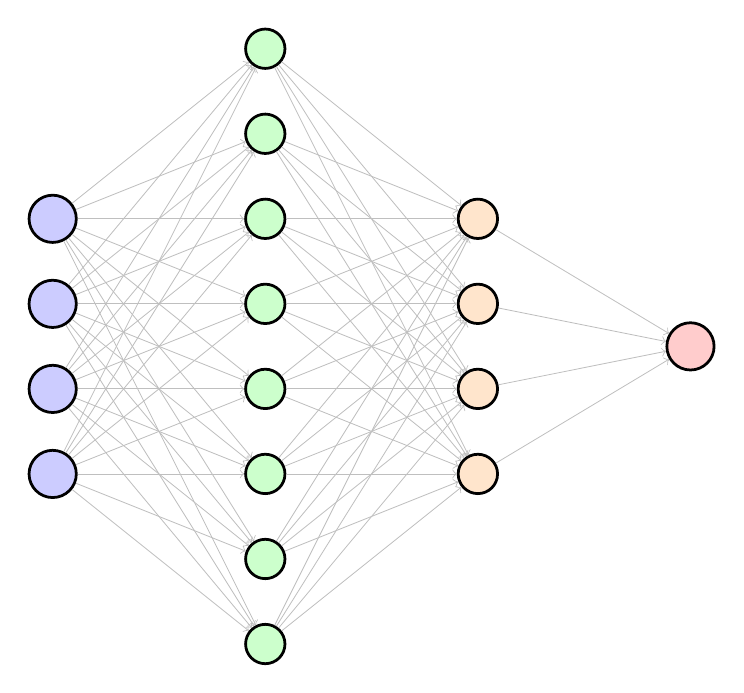
\begin{tikzpicture}[scale=0.9]
        % 定义神经元间距
        \def\spacing{1.2}
        
        % 输入层 - 4个神经元,关于横轴对称
        \node[circle, draw, minimum size=0.6cm, fill=blue!20, line width=1pt] (x1) at (0, -1.8) {};
        \node[circle, draw, minimum size=0.6cm, fill=blue!20, line width=1pt] (x2) at (0, -0.6) {};
        \node[circle, draw, minimum size=0.6cm, fill=blue!20, line width=1pt] (x3) at (0, 0.6) {};
        \node[circle, draw, minimum size=0.6cm, fill=blue!20, line width=1pt] (x4) at (0, 1.8) {};
        
        % 隐藏层1 - 8个神经元,关于横轴对称
        \node[circle, draw, minimum size=0.5cm, fill=green!20, line width=1pt] (h11) at (3, -4.2) {};
        \node[circle, draw, minimum size=0.5cm, fill=green!20, line width=1pt] (h12) at (3, -3.0) {};
        \node[circle, draw, minimum size=0.5cm, fill=green!20, line width=1pt] (h13) at (3, -1.8) {};
        \node[circle, draw, minimum size=0.5cm, fill=green!20, line width=1pt] (h14) at (3, -0.6) {};
        \node[circle, draw, minimum size=0.5cm, fill=green!20, line width=1pt] (h15) at (3, 0.6) {};
        \node[circle, draw, minimum size=0.5cm, fill=green!20, line width=1pt] (h16) at (3, 1.8) {};
        \node[circle, draw, minimum size=0.5cm, fill=green!20, line width=1pt] (h17) at (3, 3.0) {};
        \node[circle, draw, minimum size=0.5cm, fill=green!20, line width=1pt] (h18) at (3, 4.2) {};
        
        % 隐藏层2 - 4个神经元,关于横轴对称
        \node[circle, draw, minimum size=0.5cm, fill=orange!20, line width=1pt] (h21) at (6, -1.8) {};
        \node[circle, draw, minimum size=0.5cm, fill=orange!20, line width=1pt] (h22) at (6, -0.6) {};
        \node[circle, draw, minimum size=0.5cm, fill=orange!20, line width=1pt] (h23) at (6, 0.6) {};
        \node[circle, draw, minimum size=0.5cm, fill=orange!20, line width=1pt] (h24) at (6, 1.8) {};
        
        % 输出层 - 1个神经元,在横轴上
        \node[circle, draw, minimum size=0.6cm, fill=red!20, line width=1pt] (y) at (9, 0) {};
        
        % 输入层到隐藏层1的连接
        \foreach \i in {1,...,4}
            \foreach \j in {1,...,8}
                \draw[->, gray!50, line width=0.3pt] (x\i) -- (h1\j);
        
        % 隐藏层1到隐藏层2的连接
        \foreach \i in {1,...,8}
            \foreach \j in {1,...,4}
                \draw[->, gray!50, line width=0.3pt] (h1\i) -- (h2\j);
        
        % 隐藏层2到输出层的连接
        \foreach \i in {1,...,4}
            \draw[->, gray!50, line width=0.3pt] (h2\i) -- (y);
        \end{tikzpicture}
        
        \vfill
        \vspace{2cm}
        {\normalsize #5}
        \vspace{1.5cm}
    \end{center}
    \newpage
}



% 页眉页脚设置
\pagestyle{fancy}
\fancyhf{}
\fancyhead[L]{\leftmark}
\fancyhead[R]{\thepage}
\fancyfoot[C]{\small 大语言模型核心理论与应用}
\renewcommand{\headrulewidth}{0.3pt}
\renewcommand{\footrulewidth}{0.3pt}

\title{大语言模型核心理论与应用}
\author{}
\date{\today}

\newtheorem{definition}{定义}[section]
\newtheorem{theorem}{定理}[section]
\newtheorem{example}{例}[section]
\newtheorem{remark}{注}[section]

\begin{document}

% 封面
\makecover{大语言模型核心理论与应用}{Transformer · 注意力机制 · 预训练微调 · 提示工程 · RAG}{从基础架构到高级应用,全面掌握大语言模型技术}{AI/ML 系列教程}

\maketitle

\tableofcontents
\newpage

\section{引言}

大语言模型(Large Language Model, LLM)是基于深度学习的自然语言处理模型,通过在大规模文本数据上预训练,学习语言的统计规律和语义表示,展现出强大的语言理解和生成能力。从 GPT 系列到 BERT,从 Transformer 架构到注意力机制,大语言模型已经成为人工智能领域最活跃的研究方向之一。

\textbf{大语言模型的核心优势}:
\begin{itemize}
    \item \textbf{零样本学习能力}:无需针对特定任务进行训练,即可完成多种任务
    \item \textbf{通用性}:同一个模型可以应用于多种不同的 NLP 任务
    \item \textbf{自然语言理解}:能够理解复杂的语义关系和上下文
    \item \textbf{上下文学习}:通过 few-shot 或 in-context learning 快速适应新任务
    \item \textbf{可扩展性}:模型规模越大,性能通常越好
\end{itemize}

\textbf{大语言模型面临的挑战}:
\begin{itemize}
    \item \textbf{准确性}:可能产生错误或虚假信息(幻觉问题)
    \item \textbf{实时性}:推理速度可能较慢,难以满足实时应用需求
    \item \textbf{成本}:训练和部署成本高昂,需要大量计算资源
    \item \textbf{数据隐私}:训练数据可能包含敏感信息
    \item \textbf{可解释性}:模型决策过程缺乏可解释性
    \item \textbf{偏见和公平性}:可能学习并放大训练数据中的偏见
\end{itemize}

本文档分为两部分:第一部分介绍与深度学习、机器学习结合较紧密的基础内容,包括 PyTorch 框架、Transformer 架构、注意力机制等;第二部分介绍较独立和先进的知识与技术,包括预训练与微调、提示工程、RAG、代码生成等。

\part{第一部分:基础概念与框架}

\section{PyTorch 基础框架}

PyTorch 是 Facebook 开发的深度学习框架,以其动态计算图和易用性成为大语言模型开发的首选工具。

\subsection{PyTorch 核心概念}

\textbf{张量(Tensor)}:PyTorch 的基本数据结构,类似于 NumPy 数组,但支持 GPU 加速。

\begin{lstlisting}[caption=PyTorch 张量基础操作]
import torch

# 创建张量
x = torch.tensor([1, 2, 3])  # 一维张量
y = torch.randn(3, 4)        # 3x4 随机张量
z = torch.zeros(2, 3)        # 2x3 零张量

# 张量运算
a = torch.tensor([[1, 2], [3, 4]])
b = torch.tensor([[5, 6], [7, 8]])
c = torch.matmul(a, b)       # 矩阵乘法
d = a + b                    # 逐元素加法

# GPU 支持
device = torch.device('cuda' if torch.cuda.is_available() else 'cpu')
x_gpu = x.to(device)
\end{lstlisting}

\textbf{自动微分(Autograd)}:PyTorch 的自动微分系统,用于计算梯度。

\begin{lstlisting}[caption=自动微分示例]
import torch

x = torch.tensor(2.0, requires_grad=True)
y = x ** 2 + 3 * x + 1
y.backward()  # 反向传播
print(x.grad)  # 输出: tensor(7.) = 2*x + 3 (在 x=2 处)
\end{lstlisting}

\textbf{神经网络模块(nn.Module)}:PyTorch 中定义神经网络的基础类。

\begin{lstlisting}[caption=简单的神经网络定义]
import torch
import torch.nn as nn

class SimpleNet(nn.Module):
    def __init__(self, input_size, hidden_size, output_size):
        super(SimpleNet, self).__init__()
        self.fc1 = nn.Linear(input_size, hidden_size)
        self.relu = nn.ReLU()
        self.fc2 = nn.Linear(hidden_size, output_size)
    
    def forward(self, x):
        x = self.fc1(x)
        x = self.relu(x)
        x = self.fc2(x)
        return x

# 使用模型
model = SimpleNet(784, 128, 10)
x = torch.randn(32, 784)  # 批量大小 32
output = model(x)
\end{lstlisting}

\subsection{PyTorch 常用 API}

\textbf{nn.Linear}:全连接层
\begin{lstlisting}
linear = nn.Linear(in_features=768, out_features=3072)
# 输入: (batch_size, 768)
# 输出: (batch_size, 3072)
\end{lstlisting}

\textbf{nn.Embedding}:词嵌入层
\begin{lstlisting}
embedding = nn.Embedding(num_embeddings=50000, embedding_dim=768)
# 输入: (batch_size, seq_len) - 整数索引
# 输出: (batch_size, seq_len, 768) - 嵌入向量
\end{lstlisting}

\textbf{nn.LayerNorm}:层归一化
\begin{lstlisting}
layer_norm = nn.LayerNorm(normalized_shape=768)
# 输入: (batch_size, seq_len, 768)
# 输出: (batch_size, seq_len, 768)
\end{lstlisting}

\textbf{nn.Dropout}:Dropout 层
\begin{lstlisting}
dropout = nn.Dropout(p=0.1)
# 训练时随机丢弃 10% 的神经元
# 测试时所有神经元都参与计算
\end{lstlisting}

\textbf{nn.MultiheadAttention}:多头注意力(PyTorch 内置实现)
\begin{lstlisting}
attention = nn.MultiheadAttention(
    embed_dim=768,
    num_heads=12,
    dropout=0.1,
    batch_first=True
)
# query, key, value: (batch_size, seq_len, 768)
# output: (batch_size, seq_len, 768)
# attn_weights: (batch_size, seq_len, seq_len)
\end{lstlisting}

\section{Transformer 架构基础}

Transformer 是 Vaswani 等人在 2017 年提出的完全基于注意力机制的架构,成为现代大语言模型的基础。

\subsection{Transformer 整体架构}

Transformer 由编码器(Encoder)和解码器(Decoder)组成:

\textbf{编码器}:$N$ 个相同的层堆叠,每层包含:
\begin{itemize}
    \item 多头自注意力子层
    \item 前馈神经网络子层
    \item 残差连接和层归一化
\end{itemize}

\textbf{解码器}:$N$ 个相同的层堆叠,每层包含:
\begin{itemize}
    \item 掩码多头自注意力子层(防止看到未来信息)
    \item 编码器-解码器注意力子层
    \item 前馈神经网络子层
    \item 残差连接和层归一化
\end{itemize}

\begin{lstlisting}[caption=Transformer 编码器层实现]
import torch
import torch.nn as nn
import math

class TransformerEncoderLayer(nn.Module):
    def __init__(self, d_model, nhead, dim_feedforward, dropout=0.1):
        super().__init__()
        self.self_attn = nn.MultiheadAttention(
            d_model, nhead, dropout=dropout, batch_first=True
        )
        self.linear1 = nn.Linear(d_model, dim_feedforward)
        self.dropout = nn.Dropout(dropout)
        self.linear2 = nn.Linear(dim_feedforward, d_model)
        self.norm1 = nn.LayerNorm(d_model)
        self.norm2 = nn.LayerNorm(d_model)
        self.dropout1 = nn.Dropout(dropout)
        self.dropout2 = nn.Dropout(dropout)
    
    def forward(self, src, src_mask=None):
        # 自注意力
        src2 = self.self_attn(src, src, src, attn_mask=src_mask)[0]
        src = src + self.dropout1(src2)
        src = self.norm1(src)
        
        # 前馈网络
        src2 = self.linear2(self.dropout(torch.relu(self.linear1(src))))
        src = src + self.dropout2(src2)
        src = self.norm2(src)
        
        return src
\end{lstlisting}

\subsection{位置编码}

由于 Transformer 没有循环结构,需要显式编码位置信息。

\begin{definition}[位置编码]
对于位置 $pos$ 和维度 $i$,位置编码定义为:
\begin{align}
PE_{(pos, 2i)} &= \sin\left(\frac{pos}{10000^{2i/d_{model}}}\right) \\
PE_{(pos, 2i+1)} &= \cos\left(\frac{pos}{10000^{2i/d_{model}}}\right)
\end{align}
其中,$d_{model}$ 是模型维度。
\end{definition}

\begin{lstlisting}[caption=位置编码实现]
import torch
import torch.nn as nn
import math

class PositionalEncoding(nn.Module):
    def __init__(self, d_model, max_len=5000):
        super().__init__()
        
        pe = torch.zeros(max_len, d_model)
        position = torch.arange(0, max_len, dtype=torch.float).unsqueeze(1)
        div_term = torch.exp(torch.arange(0, d_model, 2).float() * 
                            (-math.log(10000.0) / d_model))
        pe[:, 0::2] = torch.sin(position * div_term)
        pe[:, 1::2] = torch.cos(position * div_term)
        pe = pe.unsqueeze(0)  # (1, max_len, d_model)
        self.register_buffer('pe', pe)
    
    def forward(self, x):
        # x: (batch_size, seq_len, d_model)
        x = x + self.pe[:, :x.size(1), :]
        return x
\end{lstlisting}

\section{注意力机制详解}

注意力机制(Attention Mechanism)是 Transformer 的核心创新,它允许模型在处理序列时动态关注不同位置的信息,解决了传统 RNN 无法并行计算和长距离依赖建模困难的问题。

\subsection{注意力机制的基本原理}

\subsubsection{为什么需要注意力机制?}

\textbf{传统序列模型的局限性}:
\begin{itemize}
    \item \textbf{RNN 的问题}:需要顺序计算,无法并行;长距离依赖建模困难;梯度消失/爆炸
    \item \textbf{CNN 的问题}:感受野有限,需要多层才能捕获长距离依赖
    \item \textbf{解决方案}:注意力机制可以直接建模任意距离的依赖关系,且支持并行计算
\end{itemize}

\subsubsection{注意力机制的直观理解}

\textbf{类比:信息检索系统}

想象你在图书馆查找资料:
\begin{itemize}
    \item \textbf{查询(Query, Q)}:你的问题或需求("我想找什么信息")
    \item \textbf{键(Key, K)}:每本书的索引标签("我提供什么信息")
    \item \textbf{值(Value, V)}:书中的实际内容("实际的信息内容")
    \item \textbf{注意力权重}:通过比较你的问题(Q)和书的索引(K),决定哪些书最相关,然后从这些书(V)中提取信息
\end{itemize}

\textbf{在神经网络中的应用}:
\begin{itemize}
    \item 每个位置都可以"查询"其他位置的信息
    \item 通过计算查询和键的相似度,得到注意力权重
    \item 使用注意力权重对值进行加权求和,得到该位置的输出
\end{itemize}

\subsubsection{缩放点积注意力的数学原理}

\begin{definition}[缩放点积注意力(Scaled Dot-Product Attention)]
给定查询矩阵 $\mathbf{Q} \in \mathbb{R}^{n \times d_k}$、键矩阵 $\mathbf{K} \in \mathbb{R}^{m \times d_k}$ 和值矩阵 $\mathbf{V} \in \mathbb{R}^{m \times d_v}$,缩放点积注意力计算为:

\begin{equation}
\text{Attention}(\mathbf{Q}, \mathbf{K}, \mathbf{V}) = \text{softmax}\left(\frac{\mathbf{Q}\mathbf{K}^T}{\sqrt{d_k}}\right)\mathbf{V}
\end{equation}

其中,$n$ 是查询序列长度,$m$ 是键值序列长度,$d_k$ 是键的维度,$\sqrt{d_k}$ 是缩放因子。
\end{definition}

\textbf{计算步骤详解}:

\textbf{步骤1:计算注意力分数(Attention Scores)}

对于每个查询向量 $\mathbf{q}_i$ 和键向量 $\mathbf{k}_j$,计算点积:
\begin{equation}
s_{ij} = \mathbf{q}_i \cdot \mathbf{k}_j = \mathbf{q}_i^T \mathbf{k}_j
\end{equation}

矩阵形式:
\begin{equation}
\mathbf{S} = \mathbf{Q}\mathbf{K}^T \in \mathbb{R}^{n \times m}
\end{equation}

其中,$S_{ij}$ 表示第 $i$ 个查询对第 $j$ 个键的注意力分数。

\textbf{步骤2:缩放(Scaling)}

为了防止点积值过大导致 softmax 梯度消失,除以 $\sqrt{d_k}$:
\begin{equation}
\mathbf{S}_{scaled} = \frac{\mathbf{Q}\mathbf{K}^T}{\sqrt{d_k}}
\end{equation}

\textbf{为什么需要缩放?}

当 $d_k$ 很大时,点积的值会很大,导致 softmax 函数进入饱和区域(梯度接近0)。缩放因子 $\sqrt{d_k}$ 使得点积的方差保持为1,假设 $\mathbf{Q}$ 和 $\mathbf{K}$ 的元素独立且均值为0、方差为1。

\textbf{步骤3:Softmax 归一化}

将注意力分数转换为概率分布:
\begin{equation}
\alpha_{ij} = \frac{\exp(s_{ij}/\sqrt{d_k})}{\sum_{k=1}^m \exp(s_{ik}/\sqrt{d_k})}
\end{equation}

矩阵形式:
\begin{equation}
\mathbf{A} = \text{softmax}\left(\frac{\mathbf{Q}\mathbf{K}^T}{\sqrt{d_k}}\right) \in \mathbb{R}^{n \times m}
\end{equation}

其中,$\alpha_{ij}$ 表示第 $i$ 个查询对第 $j$ 个键的注意力权重,满足 $\sum_{j=1}^m \alpha_{ij} = 1$。

\textbf{步骤4:加权求和}

使用注意力权重对值进行加权求和:
\begin{equation}
\mathbf{z}_i = \sum_{j=1}^m \alpha_{ij} \mathbf{v}_j
\end{equation}

矩阵形式:
\begin{equation}
\text{Attention}(\mathbf{Q}, \mathbf{K}, \mathbf{V}) = \mathbf{A}\mathbf{V} \in \mathbb{R}^{n \times d_v}
\end{equation}

\textbf{完整的数学表达式}:

\begin{align}
\text{Attention}(\mathbf{Q}, \mathbf{K}, \mathbf{V}) &= \text{softmax}\left(\frac{\mathbf{Q}\mathbf{K}^T}{\sqrt{d_k}}\right)\mathbf{V} \\
&= \left[\frac{\exp(\mathbf{Q}\mathbf{K}^T/\sqrt{d_k})}{\mathbf{1}_m^T \exp(\mathbf{Q}\mathbf{K}^T/\sqrt{d_k})}\right]\mathbf{V}
\end{align}

其中,$\mathbf{1}_m$ 是全1向量,分母是逐行的归一化因子。

\begin{lstlisting}[caption=缩放点积注意力详细实现(带注释)]
import torch
import torch.nn as nn
import torch.nn.functional as F
import math

def scaled_dot_product_attention(Q, K, V, mask=None):
    """
    缩放点积注意力实现
    
    参数:
        Q: 查询矩阵 (batch_size, seq_len_q, d_k)
        K: 键矩阵 (batch_size, seq_len_k, d_k)
        V: 值矩阵 (batch_size, seq_len_v, d_v)
        mask: 掩码矩阵 (batch_size, seq_len_q, seq_len_k) 或 None
             - mask[i,j] = 1 表示允许注意力
             - mask[i,j] = 0 表示禁止注意力(会被设为 -inf)
    
    返回:
        output: 注意力输出 (batch_size, seq_len_q, d_v)
        attn_weights: 注意力权重 (batch_size, seq_len_q, seq_len_k)
    """
    d_k = Q.size(-1)  # 获取键的维度
    
    # 步骤1:计算注意力分数 QK^T
    # Q: (batch_size, seq_len_q, d_k)
    # K: (batch_size, seq_len_k, d_k)
    # scores: (batch_size, seq_len_q, seq_len_k)
    scores = torch.matmul(Q, K.transpose(-2, -1))
    
    # 步骤2:缩放,除以 sqrt(d_k)
    # 防止点积值过大,避免 softmax 梯度消失
    scores = scores / math.sqrt(d_k)
    
    # 步骤3:应用掩码(如果有)
    # 将掩码为0的位置设为很大的负数,softmax后接近0
    if mask is not None:
        scores = scores.masked_fill(mask == 0, -1e9)
    
    # 步骤4:Softmax 归一化,得到注意力权重
    # attn_weights[i,j] 表示第i个查询对第j个键的注意力权重
    attn_weights = F.softmax(scores, dim=-1)
    
    # 步骤5:加权求和,使用注意力权重对值进行加权
    # attn_weights: (batch_size, seq_len_q, seq_len_k)
    # V: (batch_size, seq_len_k, d_v)
    # output: (batch_size, seq_len_q, d_v)
    output = torch.matmul(attn_weights, V)
    
    return output, attn_weights

# 使用示例
batch_size = 2
seq_len_q = 5  # 查询序列长度
seq_len_k = 5  # 键值序列长度
d_k = 64       # 键的维度
d_v = 64       # 值的维度

Q = torch.randn(batch_size, seq_len_q, d_k)
K = torch.randn(batch_size, seq_len_k, d_k)
V = torch.randn(batch_size, seq_len_k, d_v)

# 计算注意力
output, attn_weights = scaled_dot_product_attention(Q, K, V)

print(f"输入 Q 形状: {Q.shape}")
print(f"输入 K 形状: {K.shape}")
print(f"输入 V 形状: {V.shape}")
print(f"输出形状: {output.shape}")
print(f"注意力权重形状: {attn_weights.shape}")
print(f"注意力权重每行和: {attn_weights.sum(dim=-1)}")  # 应该接近1
\end{lstlisting}

\textbf{时间复杂度分析}:

对于序列长度 $n$ 和维度 $d$:
\begin{itemize}
    \item \textbf{计算 $\mathbf{Q}\mathbf{K}^T$}:$O(n^2 \cdot d)$
    \item \textbf{Softmax}:$O(n^2)$
    \item \textbf{加权求和 $\mathbf{A}\mathbf{V}$}:$O(n^2 \cdot d)$
    \item \textbf{总复杂度}:$O(n^2 \cdot d)$
\end{itemize}

注意:注意力机制的复杂度是序列长度的平方,这是 Transformer 的主要计算瓶颈。

\subsection{自注意力机制(Self-Attention)}

\subsubsection{自注意力的定义}

自注意力(Self-Attention)是查询、键和值都来自同一输入序列的注意力机制。也就是说,序列中的每个位置都可以"查询"序列中所有位置(包括自己)的信息。

\begin{definition}[自注意力]
对于输入序列 $\mathbf{X} \in \mathbb{R}^{n \times d}$,自注意力计算为:
\begin{equation}
\mathbf{Z} = \text{Attention}(\mathbf{X}\mathbf{W}_Q, \mathbf{X}\mathbf{W}_K, \mathbf{X}\mathbf{W}_V)
\end{equation}

其中:
\begin{itemize}
    \item $\mathbf{W}_Q \in \mathbb{R}^{d \times d_k}$:查询投影矩阵
    \item $\mathbf{W}_K \in \mathbb{R}^{d \times d_k}$:键投影矩阵
    \item $\mathbf{W}_V \in \mathbb{R}^{d \times d_v}$:值投影矩阵
    \item $\mathbf{Z} \in \mathbb{R}^{n \times d_v}$:自注意力输出
\end{itemize}
\end{definition}

\subsubsection{自注意力的计算过程}

\textbf{步骤详解}:

\textbf{步骤1:生成 Q、K、V}

对于输入序列 $\mathbf{X} = [\mathbf{x}_1, \mathbf{x}_2, \ldots, \mathbf{x}_n]^T$:
\begin{align}
\mathbf{Q} &= \mathbf{X}\mathbf{W}_Q = [\mathbf{q}_1, \mathbf{q}_2, \ldots, \mathbf{q}_n]^T \\
\mathbf{K} &= \mathbf{X}\mathbf{W}_K = [\mathbf{k}_1, \mathbf{k}_2, \ldots, \mathbf{k}_n]^T \\
\mathbf{V} &= \mathbf{X}\mathbf{W}_V = [\mathbf{v}_1, \mathbf{v}_2, \ldots, \mathbf{v}_n]^T
\end{align}

\textbf{步骤2:计算注意力权重}

对于位置 $i$,计算它对所有位置的注意力权重:
\begin{equation}
\alpha_{ij} = \frac{\exp(\mathbf{q}_i^T \mathbf{k}_j / \sqrt{d_k})}{\sum_{k=1}^n \exp(\mathbf{q}_i^T \mathbf{k}_k / \sqrt{d_k})}
\end{equation}

\textbf{步骤3:加权求和}

位置 $i$ 的输出是所有位置的值的加权和:
\begin{equation}
\mathbf{z}_i = \sum_{j=1}^n \alpha_{ij} \mathbf{v}_j
\end{equation}

\textbf{矩阵形式}:
\begin{equation}
\mathbf{Z} = \text{softmax}\left(\frac{\mathbf{X}\mathbf{W}_Q (\mathbf{X}\mathbf{W}_K)^T}{\sqrt{d_k}}\right) \mathbf{X}\mathbf{W}_V
\end{equation}

\subsubsection{自注意力的优势}

\textbf{1. 并行计算}:
\begin{itemize}
    \item 所有位置的 Q、K、V 可以并行计算
    \item 所有位置的注意力输出可以并行计算
    \item 时间复杂度:$O(n^2 \cdot d)$,但可以完全并行
    \item 相比 RNN 的 $O(n \cdot d^2)$ 顺序计算,虽然复杂度更高,但并行度更高
\end{itemize}

\textbf{2. 长距离依赖}:
\begin{itemize}
    \item 可以直接建模任意距离的依赖关系
    \item 不需要像 RNN 那样通过多步传播
    \item 不需要像 CNN 那样通过多层堆叠
\end{itemize}

\textbf{3. 可解释性}:
\begin{itemize}
    \item 注意力权重 $\alpha_{ij}$ 可以可视化
    \item 可以看到模型在关注哪些位置
    \item 有助于理解模型的决策过程
\end{itemize}

\begin{lstlisting}[caption=自注意力详细实现(带注释)]
import torch
import torch.nn as nn
import torch.nn.functional as F
import math

class SelfAttention(nn.Module):
    """
    自注意力模块
    
    参数:
        d_model: 输入和输出的维度
        d_k: 键和查询的维度(默认等于 d_model)
        d_v: 值的维度(默认等于 d_model)
    """
    def __init__(self, d_model, d_k=None, d_v=None):
        super().__init__()
        if d_k is None:
            d_k = d_model
        if d_v is None:
            d_v = d_model
        
        # 定义三个线性投影层
        # 将输入 x 投影到 Q、K、V 空间
        self.W_q = nn.Linear(d_model, d_k)  # 查询投影
        self.W_k = nn.Linear(d_model, d_k)  # 键投影
        self.W_v = nn.Linear(d_model, d_v)  # 值投影
        self.d_k = d_k
    
    def forward(self, x, mask=None):
        """
        前向传播
        
        参数:
            x: 输入序列 (batch_size, seq_len, d_model)
            mask: 掩码矩阵 (batch_size, seq_len, seq_len) 或 None
        
        返回:
            output: 自注意力输出 (batch_size, seq_len, d_v)
            attn_weights: 注意力权重 (batch_size, seq_len, seq_len)
        """
        batch_size, seq_len, d_model = x.size()
        
        # 步骤1:通过线性投影生成 Q、K、V
        # 所有位置共享相同的投影矩阵
        Q = self.W_q(x)  # (batch_size, seq_len, d_k)
        K = self.W_k(x)  # (batch_size, seq_len, d_k)
        V = self.W_v(x)  # (batch_size, seq_len, d_v)
        
        # 步骤2:计算缩放点积注意力
        output, attn_weights = scaled_dot_product_attention(Q, K, V, mask)
        
        return output, attn_weights

# 使用示例
d_model = 512
seq_len = 10
batch_size = 2

# 创建自注意力模块
self_attn = SelfAttention(d_model=d_model)

# 创建输入(随机初始化)
x = torch.randn(batch_size, seq_len, d_model)

# 前向传播
output, attn_weights = self_attn(x)

print(f"输入形状: {x.shape}")
print(f"输出形状: {output.shape}")
print(f"注意力权重形状: {attn_weights.shape}")
print(f"注意力权重示例(第一个样本,第一个位置):")
print(attn_weights[0, 0, :])  # 第一个样本,第一个位置对所有位置的注意力
print(f"注意力权重和: {attn_weights[0, 0, :].sum()}")  # 应该接近1
\end{lstlisting}


\subsection{多头注意力机制(Multi-Head Attention)}

\subsubsection{为什么需要多头注意力?}

\textbf{单头注意力的局限性}:
\begin{itemize}
    \item 只有一个注意力头,只能学习一种类型的依赖关系
    \item 表达能力有限,难以同时捕获多种语义关系
    \item 例如:语法关系、语义关系、位置关系等
\end{itemize}

\textbf{多头注意力的优势}:
\begin{itemize}
    \item \textbf{多视角学习}:不同头可以关注不同的关系类型
    \item \textbf{表达能力增强}:通过多个子空间学习,增强模型表达能力
    \item \textbf{并行计算}:多个头可以并行计算,提高效率
    \item \textbf{专业化}:不同头可以学习不同的模式(如语法、语义、位置等)
\end{itemize}

\subsubsection{多头注意力的数学原理}

\begin{definition}[多头注意力]
多头注意力使用 $h$ 个注意力头并行计算,每个头在不同的表示子空间中学习:

\begin{align}
\text{MultiHead}(\mathbf{Q}, \mathbf{K}, \mathbf{V}) &= \text{Concat}(\text{head}_1, \ldots, \text{head}_h) \mathbf{W}^O \\
\text{head}_i &= \text{Attention}(\mathbf{Q}\mathbf{W}_i^Q, \mathbf{K}\mathbf{W}_i^K, \mathbf{V}\mathbf{W}_i^V)
\end{align}

其中:
\begin{itemize}
    \item $h$ 是注意力头的数量(通常取 8、12、16 等)
    \item $\mathbf{W}_i^Q \in \mathbb{R}^{d_{model} \times d_k}$:第 $i$ 个头的查询投影矩阵
    \item $\mathbf{W}_i^K \in \mathbb{R}^{d_{model} \times d_k}$:第 $i$ 个头的键投影矩阵
    \item $\mathbf{W}_i^V \in \mathbb{R}^{d_{model} \times d_v}$:第 $i$ 个头的值投影矩阵
    \item $\mathbf{W}^O \in \mathbb{R}^{h \cdot d_v \times d_{model}}$:输出投影矩阵
    \item $d_k = d_v = d_{model} / h$:每个头的维度
\end{itemize}
\end{definition}

\textbf{维度关系}:

假设 $d_{model} = 512$,$h = 8$:
\begin{itemize}
    \item 每个头的维度:$d_k = d_v = 512 / 8 = 64$
    \item 所有头拼接后:$h \cdot d_v = 8 \times 64 = 512$
    \item 输出投影后:$512 \times 512$,保持维度不变
\end{itemize}

\textbf{计算过程详解}:

\textbf{步骤1:为每个头生成 Q、K、V}

对于输入 $\mathbf{X} \in \mathbb{R}^{n \times d_{model}}$,首先通过共享的线性投影:
\begin{align}
\mathbf{Q} &= \mathbf{X}\mathbf{W}_Q \in \mathbb{R}^{n \times d_{model}} \\
\mathbf{K} &= \mathbf{X}\mathbf{W}_K \in \mathbb{R}^{n \times d_{model}} \\
\mathbf{V} &= \mathbf{X}\mathbf{W}_V \in \mathbb{R}^{n \times d_{model}}
\end{align}

然后将 $\mathbf{Q}$、$\mathbf{K}$、$\mathbf{V}$ 重塑并分割为 $h$ 个头:
\begin{align}
\mathbf{Q} &\rightarrow [\mathbf{Q}_1, \mathbf{Q}_2, \ldots, \mathbf{Q}_h], \quad \mathbf{Q}_i \in \mathbb{R}^{n \times d_k} \\
\mathbf{K} &\rightarrow [\mathbf{K}_1, \mathbf{K}_2, \ldots, \mathbf{K}_h], \quad \mathbf{K}_i \in \mathbb{R}^{n \times d_k} \\
\mathbf{V} &\rightarrow [\mathbf{V}_1, \mathbf{V}_2, \ldots, \mathbf{V}_h], \quad \mathbf{V}_i \in \mathbb{R}^{n \times d_v}
\end{align}

\textbf{步骤2:每个头独立计算注意力}

对于第 $i$ 个头:
\begin{equation}
\text{head}_i = \text{Attention}(\mathbf{Q}_i, \mathbf{K}_i, \mathbf{V}_i) \in \mathbb{R}^{n \times d_v}
\end{equation}

\textbf{步骤3:拼接所有头}

\begin{equation}
\text{Concat}(\text{head}_1, \ldots, \text{head}_h) \in \mathbb{R}^{n \times (h \cdot d_v)} = \mathbb{R}^{n \times d_{model}}
\end{equation}

\textbf{步骤4:输出投影}

\begin{equation}
\text{MultiHead}(\mathbf{Q}, \mathbf{K}, \mathbf{V}) = \text{Concat}(\text{head}_1, \ldots, \text{head}_h) \mathbf{W}^O \in \mathbb{R}^{n \times d_{model}}
\end{equation}

\subsubsection{如何实现多头注意力?}

\textbf{实现策略}:

有两种实现多头注意力的方式:

\textbf{方式1:为每个头单独定义投影矩阵}(理论方式,不常用)
\begin{itemize}
    \item 为每个头定义独立的 $\mathbf{W}_i^Q$、$\mathbf{W}_i^K$、$\mathbf{W}_i^V$
    \item 参数量:$h \times (d_{model} \times d_k + d_{model} \times d_k + d_{model} \times d_v)$
    \item 优点:每个头完全独立
    \item 缺点:参数量大,实现复杂
\end{itemize}

\textbf{方式2:共享投影矩阵,然后分割}(实际使用的方式)
\begin{itemize}
    \item 使用共享的 $\mathbf{W}_Q$、$\mathbf{W}_K$、$\mathbf{W}_V$ 投影到 $d_{model}$ 维
    \item 然后将结果重塑并分割为 $h$ 个头
    \item 参数量:$d_{model} \times d_{model} \times 3 + d_{model} \times d_{model}$(更少)
    \item 优点:参数量少,实现简单,效果相同
\end{itemize}

\textbf{维度变换详解}:

假设 $d_{model} = 512$,$h = 8$,$d_k = d_v = 64$,序列长度 $n = 10$:

\textbf{步骤1:共享线性投影}
\begin{align}
\mathbf{Q} &= \mathbf{X}\mathbf{W}_Q \in \mathbb{R}^{10 \times 512} \\
\mathbf{K} &= \mathbf{X}\mathbf{W}_K \in \mathbb{R}^{10 \times 512} \\
\mathbf{V} &= \mathbf{X}\mathbf{W}_V \in \mathbb{R}^{10 \times 512}
\end{align}

\textbf{步骤2:重塑为多头形式}

将 $\mathbf{Q}$ 重塑为 $(n, h, d_k)$:
\begin{equation}
\mathbf{Q} \in \mathbb{R}^{10 \times 512} \rightarrow \mathbf{Q}' \in \mathbb{R}^{10 \times 8 \times 64}
\end{equation}

然后转置为 $(h, n, d_k)$ 以便并行计算:
\begin{equation}
\mathbf{Q}' \in \mathbb{R}^{10 \times 8 \times 64} \rightarrow \mathbf{Q}'' \in \mathbb{R}^{8 \times 10 \times 64}
\end{equation}

这样,$\mathbf{Q}''[i]$ 就是第 $i$ 个头的查询矩阵 $\mathbf{Q}_i \in \mathbb{R}^{10 \times 64}$。

\textbf{步骤3:并行计算所有头的注意力}

对于每个头 $i$:
\begin{equation}
\text{head}_i = \text{Attention}(\mathbf{Q}_i, \mathbf{K}_i, \mathbf{V}_i) \in \mathbb{R}^{10 \times 64}
\end{equation}

所有头的结果:$\text{head}_1, \text{head}_2, \ldots, \text{head}_8$,每个都是 $\mathbb{R}^{10 \times 64}$。

\textbf{步骤4:拼接所有头}

将 $h$ 个头的结果拼接:
\begin{equation}
\text{Concat}(\text{head}_1, \ldots, \text{head}_8) \in \mathbb{R}^{10 \times 512}
\end{equation}

\textbf{步骤5:输出投影}

\begin{equation}
\text{output} = \text{Concat}(\text{head}_1, \ldots, \text{head}_8) \mathbf{W}^O \in \mathbb{R}^{10 \times 512}
\end{equation}

\begin{lstlisting}[caption=多头注意力详细实现(带完整注释)]
import torch
import torch.nn as nn
import torch.nn.functional as F
import math

class MultiHeadAttention(nn.Module):
    """
    多头注意力模块
    
    参数:
        d_model: 模型维度(输入和输出的维度)
        num_heads: 注意力头的数量
    """
    def __init__(self, d_model, num_heads):
        super().__init__()
        # 确保 d_model 可以被 num_heads 整除
        assert d_model % num_heads == 0, "d_model 必须能被 num_heads 整除"
        
        self.d_model = d_model      # 模型维度,如 512
        self.num_heads = num_heads  # 注意力头数量,如 8
        self.d_k = d_model // num_heads  # 每个头的维度,如 512 // 8 = 64
        
        # 步骤1:定义共享的线性投影层
        # 这些投影层将输入投影到 d_model 维,然后会被分割为多个头
        self.W_q = nn.Linear(d_model, d_model)  # 查询投影
        self.W_k = nn.Linear(d_model, d_model)  # 键投影
        self.W_v = nn.Linear(d_model, d_model)  # 值投影
        
        # 输出投影层,将拼接后的多头结果投影回 d_model 维
        self.W_o = nn.Linear(d_model, d_model)
    
    def forward(self, Q, K, V, mask=None):
        """
        前向传播
        
        参数:
            Q: 查询矩阵 (batch_size, seq_len_q, d_model)
            K: 键矩阵 (batch_size, seq_len_k, d_model)
            V: 值矩阵 (batch_size, seq_len_v, d_model)
            mask: 掩码矩阵 (batch_size, seq_len_q, seq_len_k) 或 None
        
        返回:
            output: 多头注意力输出 (batch_size, seq_len_q, d_model)
            attn_weights: 注意力权重 (batch_size, num_heads, seq_len_q, seq_len_k)
        """
        batch_size = Q.size(0)
        seq_len_q = Q.size(1)
        seq_len_k = K.size(1)
        
        # ========== 步骤1:共享线性投影 ==========
        # 将 Q、K、V 投影到 d_model 维
        # Q_proj: (batch_size, seq_len_q, d_model)
        # K_proj: (batch_size, seq_len_k, d_model)
        # V_proj: (batch_size, seq_len_v, d_model)
        Q_proj = self.W_q(Q)
        K_proj = self.W_k(K)
        V_proj = self.W_v(V)
        
        # ========== 步骤2:重塑为多头形式 ==========
        # 将 d_model 维分割为 num_heads 个头,每个头 d_k 维
        # 
        # 例如:d_model=512, num_heads=8, d_k=64
        # Q_proj: (batch_size, seq_len_q, 512)
        #   -> view: (batch_size, seq_len_q, 8, 64)
        #   -> transpose(1,2): (batch_size, 8, seq_len_q, 64)
        #
        # 这样 Q_multi[i] 就是第 i 个头的查询矩阵
        Q_multi = Q_proj.view(batch_size, seq_len_q, self.num_heads, self.d_k).transpose(1, 2)
        K_multi = K_proj.view(batch_size, seq_len_k, self.num_heads, self.d_k).transpose(1, 2)
        V_multi = V_proj.view(batch_size, seq_len_k, self.num_heads, self.d_k).transpose(1, 2)
        # Q_multi: (batch_size, num_heads, seq_len_q, d_k)
        # K_multi: (batch_size, num_heads, seq_len_k, d_k)
        # V_multi: (batch_size, num_heads, seq_len_k, d_k)
        
        # ========== 步骤3:并行计算所有头的注意力 ==========
        # 使用批量矩阵乘法,同时计算所有头的注意力
        # 
        # 计算注意力分数:QK^T
        # Q_multi: (batch_size, num_heads, seq_len_q, d_k)
        # K_multi: (batch_size, num_heads, seq_len_k, d_k)
        # scores: (batch_size, num_heads, seq_len_q, seq_len_k)
        scores = torch.matmul(Q_multi, K_multi.transpose(-2, -1)) / math.sqrt(self.d_k)
        
        # 应用掩码(如果有)
        if mask is not None:
            # mask: (batch_size, seq_len_q, seq_len_k)
            # 需要扩展维度以匹配 scores 的形状
            mask = mask.unsqueeze(1)  # (batch_size, 1, seq_len_q, seq_len_k)
            scores = scores.masked_fill(mask == 0, -1e9)
        
        # Softmax 归一化,得到注意力权重
        attn_weights = F.softmax(scores, dim=-1)
        # attn_weights: (batch_size, num_heads, seq_len_q, seq_len_k)
        
        # 加权求和:注意力权重 × 值
        # attn_weights: (batch_size, num_heads, seq_len_q, seq_len_k)
        # V_multi: (batch_size, num_heads, seq_len_k, d_k)
        # attn_output: (batch_size, num_heads, seq_len_q, d_k)
        attn_output = torch.matmul(attn_weights, V_multi)
        
        # ========== 步骤4:拼接所有头 ==========
        # 将多个头的结果拼接在一起
        # 
        # attn_output: (batch_size, num_heads, seq_len_q, d_k)
        #   -> transpose(1,2): (batch_size, seq_len_q, num_heads, d_k)
        #   -> contiguous().view: (batch_size, seq_len_q, num_heads * d_k)
        #   = (batch_size, seq_len_q, d_model)
        attn_output = attn_output.transpose(1, 2).contiguous().view(
            batch_size, seq_len_q, self.d_model
        )
        # attn_output: (batch_size, seq_len_q, d_model)
        
        # ========== 步骤5:输出投影 ==========
        # 将拼接后的结果投影回 d_model 维
        output = self.W_o(attn_output)
        # output: (batch_size, seq_len_q, d_model)
        
        return output, attn_weights

# ========== 使用示例 ==========
d_model = 512
num_heads = 8
seq_len = 10
batch_size = 2

# 创建多头注意力模块
multi_head_attn = MultiHeadAttention(d_model=d_model, num_heads=num_heads)

# 创建输入(Q、K、V 可以相同,也可以不同)
Q = torch.randn(batch_size, seq_len, d_model)
K = torch.randn(batch_size, seq_len, d_model)
V = torch.randn(batch_size, seq_len, d_model)

# 前向传播
output, attn_weights = multi_head_attn(Q, K, V)

print(f"输入 Q 形状: {Q.shape}")
print(f"输入 K 形状: {K.shape}")
print(f"输入 V 形状: {V.shape}")
print(f"输出形状: {output.shape}")
print(f"注意力权重形状: {attn_weights.shape}")  # (batch_size, num_heads, seq_len, seq_len)
print(f"每个头的维度 d_k: {multi_head_attn.d_k}")
print(f"注意力权重示例(第一个样本,第一个头,第一个位置):")
print(attn_weights[0, 0, 0, :])  # 第一个样本,第一个头,第一个位置对所有位置的注意力
print(f"注意力权重和: {attn_weights[0, 0, 0, :].sum()}")  # 应该接近1
\end{lstlisting}

\subsubsection{多头注意力的维度变换可视化}

\textbf{维度变换流程}(以 $d_{model}=512$,$h=8$,$d_k=64$ 为例):

\begin{center}
输入 $\mathbf{X}$: $(batch, seq, 512)$ \\
$\downarrow$ 线性投影 \\
$\mathbf{Q}$: $(batch, seq, 512)$ \\
$\downarrow$ 重塑 \\
$\mathbf{Q}'$: $(batch, seq, 8, 64)$ \\
$\downarrow$ 转置 \\
$\mathbf{Q}''$: $(batch, 8, seq, 64)$ \\
$\downarrow$ 并行计算 \\
$\text{head}_1, \ldots, \text{head}_8$: 每个 $(batch, seq, 64)$ \\
$\downarrow$ 拼接 \\
$\text{Concat}$: $(batch, seq, 512)$ \\
$\downarrow$ 输出投影 \\
输出: $(batch, seq, 512)$
\end{center}

\textbf{关键点}:
\begin{itemize}
    \item \textbf{共享投影}:所有头共享 $\mathbf{W}_Q$、$\mathbf{W}_K$、$\mathbf{W}_V$,参数量更少
    \item \textbf{分割策略}:通过 reshape 和 transpose 将 $d_{model}$ 维分割为 $h$ 个 $d_k$ 维的头
    \item \textbf{并行计算}:所有头的注意力可以并行计算,提高效率
    \item \textbf{拼接和投影}:拼接所有头的结果,然后通过 $\mathbf{W}^O$ 投影回原始维度
\end{itemize}

\subsubsection{多头注意力的优势和应用}

\textbf{优势}:

\textbf{1. 多视角学习}:
\begin{itemize}
    \item 不同头可以关注不同的关系类型
    \item 例如:头1关注语法关系,头2关注语义关系,头3关注位置关系等
    \item 通过可视化注意力权重可以观察到这种现象
\end{itemize}

\textbf{2. 表达能力增强}:
\begin{itemize}
    \item 通过多个子空间学习,增强模型表达能力
    \item 相当于从多个角度理解输入序列
    \item 比单头注意力有更强的拟合能力
\end{itemize}

\textbf{3. 并行计算}:
\begin{itemize}
    \item 多个头可以完全并行计算
    \item 时间复杂度:$O(n^2 \cdot d)$(与单头相同)
    \item 但可以充分利用 GPU 的并行计算能力
\end{itemize}

\textbf{4. 参数量优化}:
\begin{itemize}
    \item 使用共享投影矩阵,参数量为 $O(d_{model}^2)$
    \item 如果为每个头单独定义投影矩阵,参数量为 $O(h \cdot d_{model}^2)$
    \item 共享投影既减少了参数量,又保持了表达能力
\end{itemize}

\textbf{实际应用中的观察}:

研究表明,在训练好的 Transformer 模型中:
\begin{itemize}
    \item 不同头确实学习到了不同的模式
    \item 有些头关注局部依赖(相邻位置)
    \item 有些头关注长距离依赖(远距离位置)
    \item 有些头关注特定类型的语法或语义关系
\end{itemize}

\textbf{头数量的选择}:
\begin{itemize}
    \item \textbf{常见配置}:$h = 8$(BERT-base)、$h = 12$(BERT-large)、$h = 16$(GPT-3)
    \item \textbf{原则}:$d_{model}$ 必须能被 $h$ 整除
    \item \textbf{权衡}:头数越多,表达能力越强,但计算量也越大
    \item \textbf{经验}:通常 $h = 8$ 或 $h = 16$ 效果较好
\end{itemize}

\section{完整的 Transformer 实现}

本节提供一个简化的 Transformer 编码器实现,展示如何将各个组件组合起来。

\begin{lstlisting}[caption=完整的 Transformer 编码器]
import torch
import torch.nn as nn
import math

class TransformerEncoder(nn.Module):
    def __init__(self, vocab_size, d_model=512, nhead=8, 
                 num_layers=6, dim_feedforward=2048, 
                 max_seq_length=5000, dropout=0.1):
        super().__init__()
        
        self.d_model = d_model
        self.embedding = nn.Embedding(vocab_size, d_model)
        self.pos_encoding = PositionalEncoding(d_model, max_seq_length)
        
        encoder_layer = nn.TransformerEncoderLayer(
            d_model=d_model,
            nhead=nhead,
            dim_feedforward=dim_feedforward,
            dropout=dropout,
            batch_first=True
        )
        self.transformer_encoder = nn.TransformerEncoder(
            encoder_layer, num_layers=num_layers
        )
        
        self.dropout = nn.Dropout(dropout)
    
    def forward(self, src, src_mask=None, src_key_padding_mask=None):
        # src: (batch_size, seq_len)
        # 词嵌入
        src = self.embedding(src) * math.sqrt(self.d_model)
        # 位置编码
        src = self.pos_encoding(src)
        src = self.dropout(src)
        
        # Transformer 编码
        output = self.transformer_encoder(
            src, 
            mask=src_mask,
            src_key_padding_mask=src_key_padding_mask
        )
        
        return output

# 使用示例
model = TransformerEncoder(
    vocab_size=10000,
    d_model=512,
    nhead=8,
    num_layers=6
)

# 输入: (batch_size=32, seq_len=128)
input_ids = torch.randint(0, 10000, (32, 128))
output = model(input_ids)
# 输出: (32, 128, 512)
\end{lstlisting}

\section{训练与推理基础}

\subsection{训练流程}

\begin{lstlisting}[caption=Transformer 训练示例]
import torch
import torch.nn as nn
from torch.utils.data import DataLoader

# 定义模型
model = TransformerEncoder(vocab_size=10000, d_model=512)
criterion = nn.CrossEntropyLoss()
optimizer = torch.optim.Adam(model.parameters(), lr=0.0001)

# 训练循环
def train_epoch(model, dataloader, criterion, optimizer, device):
    model.train()
    total_loss = 0
    
    for batch in dataloader:
        input_ids, labels = batch
        input_ids = input_ids.to(device)
        labels = labels.to(device)
        
        # 前向传播
        outputs = model(input_ids)
        
        # 计算损失(假设是语言建模任务)
        # outputs: (batch_size, seq_len, vocab_size)
        # labels: (batch_size, seq_len)
        logits = outputs.view(-1, outputs.size(-1))
        labels_flat = labels.view(-1)
        loss = criterion(logits, labels_flat)
        
        # 反向传播
        optimizer.zero_grad()
        loss.backward()
        torch.nn.utils.clip_grad_norm_(model.parameters(), max_norm=1.0)
        optimizer.step()
        
        total_loss += loss.item()
    
    return total_loss / len(dataloader)
\end{lstlisting}

\subsection{推理流程}

\begin{lstlisting}[caption=Transformer 推理示例]
def generate_text(model, tokenizer, prompt, max_length=100, temperature=1.0):
    model.eval()
    tokens = tokenizer.encode(prompt)
    
    with torch.no_grad():
        for _ in range(max_length):
            # 准备输入
            input_ids = torch.tensor([tokens]).to(device)
            
            # 前向传播
            outputs = model(input_ids)
            
            # 获取最后一个位置的 logits
            logits = outputs[0, -1, :] / temperature
            
            # 采样下一个 token
            probs = F.softmax(logits, dim=-1)
            next_token = torch.multinomial(probs, num_samples=1).item()
            
            tokens.append(next_token)
            
            # 如果生成了结束符,停止
            if next_token == tokenizer.eos_token_id:
                break
    
    return tokenizer.decode(tokens)
\end{lstlisting}

\section{总结}

第一部分介绍了大语言模型的基础概念和框架:
\begin{itemize}
    \item \textbf{PyTorch 框架}:深度学习开发的基础工具
    \item \textbf{Transformer 架构}:现代 LLM 的核心架构
    \item \textbf{注意力机制}:包括缩放点积注意力、自注意力和多头注意力
    \item \textbf{位置编码}:为序列添加位置信息
    \item \textbf{训练与推理}:基本的模型训练和文本生成流程
\end{itemize}

这些基础内容是理解和使用大语言模型的前提,与深度学习和机器学习紧密相关。在第二部分中,我们将介绍更高级的技术和应用。

\part{第二部分:高级技术与应用}

\section{预训练与微调}

预训练是大语言模型的核心,通过在大量无标注文本上学习语言表示,然后通过微调适应特定任务。

\subsection{预训练目标}

\textbf{自回归语言建模(Autoregressive Language Modeling)}:
\begin{equation}
\mathcal{L}_{LM} = -\sum_{t=1}^T \log P(x_t | x_{<t})
\end{equation}
模型从左到右预测下一个词,GPT 系列使用此目标。

\textbf{掩码语言建模(Masked Language Modeling)}:
\begin{equation}
\mathcal{L}_{MLM} = -\sum_{i \in M} \log P(x_i | \mathbf{x}_{\backslash M})
\end{equation}
随机掩码部分词,预测被掩码的词,BERT 使用此目标。

\textbf{下一句预测(Next Sentence Prediction)}:
判断两个句子是否连续,BERT 使用此辅助任务。

\begin{lstlisting}[caption=掩码语言建模实现]
import torch
import torch.nn as nn
import random

def create_masked_lm_predictions(tokens, tokenizer, mlm_probability=0.15):
    """创建掩码语言建模的标签"""
    labels = tokens.clone()
    probability_matrix = torch.full(labels.shape, mlm_probability)
    
    # 不掩码特殊 token
    special_tokens_mask = torch.tensor([
        tokenizer.get_special_tokens_mask(val, already_has_special_tokens=True)
        for val in labels.tolist()
    ], dtype=torch.bool)
    probability_matrix.masked_fill_(special_tokens_mask, value=0.0)
    
    # 80% 的时间用 [MASK] 替换
    # 10% 的时间用随机词替换
    # 10% 的时间保持原词
    masked_indices = torch.bernoulli(probability_matrix).bool()
    labels[~masked_indices] = -100  # 只计算被掩码位置的损失
    
    # 80% 替换为 [MASK]
    indices_replaced = torch.bernoulli(
        torch.full(labels.shape, 0.8)
    ).bool() & masked_indices
    tokens[indices_replaced] = tokenizer.convert_tokens_to_ids('[MASK]')
    
    # 10% 替换为随机词
    indices_random = torch.bernoulli(
        torch.full(labels.shape, 0.5)
    ).bool() & masked_indices & ~indices_replaced
    random_words = torch.randint(len(tokenizer), labels.shape, dtype=torch.long)
    tokens[indices_random] = random_words[indices_random]
    
    return tokens, labels
\end{lstlisting}

\subsection{Few-shot Learning}

Few-shot Learning 是指模型只需少量示例就能适应新任务。

\textbf{In-context Learning}:通过在提示中包含示例,让模型学习任务模式,无需更新参数。

\begin{example}[Few-shot 示例]
\textbf{任务}:情感分析

\textbf{提示}:
\begin{verbatim}
评论:这部电影太棒了!
情感:正面

评论:服务很差,不推荐。
情感:负面

评论:还可以,一般般。
情感:
\end{verbatim}

模型应该输出"中性"。
\end{example}

\subsection{微调策略}

\textbf{全参数微调}:更新所有模型参数。

\textbf{参数高效微调(Parameter-Efficient Fine-tuning)}:
\begin{itemize}
    \item \textbf{LoRA(Low-Rank Adaptation)}:只训练低秩矩阵
    \item \textbf{Adapter}:在 Transformer 层中插入小的适配器模块
    \item \textbf{Prefix Tuning}:学习可训练的前缀
\end{itemize}

\begin{lstlisting}[caption=LoRA 实现]
import torch
import torch.nn as nn

class LoRALayer(nn.Module):
    def __init__(self, in_features, out_features, rank=8, alpha=16):
        super().__init__()
        self.rank = rank
        self.alpha = alpha
        
        # LoRA 矩阵 A 和 B
        self.lora_A = nn.Parameter(torch.randn(in_features, rank))
        self.lora_B = nn.Parameter(torch.zeros(rank, out_features))
        
        # 原始权重(冻结)
        self.weight = nn.Parameter(torch.randn(in_features, out_features))
        self.weight.requires_grad = False
    
    def forward(self, x):
        # 原始输出 + LoRA 调整
        return F.linear(x, self.weight + (self.alpha / self.rank) * 
                       torch.matmul(self.lora_B, self.lora_A))

# 应用 LoRA 到线性层
class LoRALinear(nn.Module):
    def __init__(self, linear_layer, rank=8, alpha=16):
        super().__init__()
        self.original = linear_layer
        self.lora = LoRALayer(
            linear_layer.in_features,
            linear_layer.out_features,
            rank,
            alpha
        )
    
    def forward(self, x):
        return self.original(x) + self.lora(x)
\end{lstlisting}

\section{提示工程}

提示工程(Prompt Engineering)是通过设计有效的提示来引导模型生成期望的输出。

\subsection{提示设计原则}

\begin{enumerate}
    \item \textbf{明确任务}:清楚说明要完成的任务
    \item \textbf{提供示例}:Few-shot 示例帮助模型理解任务
    \item \textbf{指定格式}:明确输出格式要求
    \item \textbf{分解任务}:将复杂任务分解为子任务
\end{enumerate}

\subsection{Chain-of-Thought(CoT)}

Chain-of-Thought 通过引导模型逐步推理,提高复杂问题的解决能力。

\begin{example}[Chain-of-Thought 示例]
\textbf{问题}:一个商店有 23 个苹果。如果他们卖了 20 个,又买了 6 个,现在有多少个?

\textbf{标准提示}:
\begin{verbatim}
Q: 一个商店有 23 个苹果。如果他们卖了 20 个,又买了 6 个,现在有多少个?
A:
\end{verbatim}

\textbf{Chain-of-Thought 提示}:
\begin{verbatim}
Q: 一个商店有 23 个苹果。如果他们卖了 20 个,又买了 6 个,现在有多少个?
A: 让我们一步步思考。
商店开始有 23 个苹果。
卖了 20 个后,剩下 23 - 20 = 3 个。
又买了 6 个,现在有 3 + 6 = 9 个。
所以答案是 9。
\end{verbatim}
\end{example}

\begin{lstlisting}[caption=Chain-of-Thought 实现示例]
def generate_cot_prompt(question, examples=None):
    """生成 Chain-of-Thought 提示"""
    prompt = "让我们一步步思考并解决这个问题。\n\n"
    
    if examples:
        for ex_q, ex_a in examples:
            prompt += f"问题:{ex_q}\n"
            prompt += f"解答:{ex_a}\n\n"
    
    prompt += f"问题:{question}\n"
    prompt += "解答:"
    return prompt

# 使用示例
question = "如果一本书有 300 页,每天读 25 页,需要多少天读完?"
cot_prompt = generate_cot_prompt(question)
# 模型会生成逐步推理过程
\end{lstlisting}

\subsection{Few-shot Prompting}

Few-shot Prompting 通过在提示中包含多个示例,让模型学习任务模式。

\begin{lstlisting}[caption=Few-shot Prompting 实现]
def create_few_shot_prompt(task_description, examples, query):
    """创建 Few-shot 提示"""
    prompt = f"{task_description}\n\n"
    
    for i, (input_ex, output_ex) in enumerate(examples, 1):
        prompt += f"示例 {i}:\n"
        prompt += f"输入:{input_ex}\n"
        prompt += f"输出:{output_ex}\n\n"
    
    prompt += f"输入:{query}\n"
    prompt += "输出:"
    return prompt

# 使用示例:情感分析
task = "对以下评论进行情感分析,输出'正面'、'负面'或'中性'。"
examples = [
    ("这部电影很棒!", "正面"),
    ("服务很差。", "负面"),
    ("还可以吧。", "中性")
]
query = "这个产品一般般。"
prompt = create_few_shot_prompt(task, examples, query)
\end{lstlisting}

\section{检索增强生成(RAG)}

RAG(Retrieval-Augmented Generation)通过检索外部知识库来增强生成,提高准确性和可追溯性。

\subsection{RAG 架构}

RAG 包含两个主要组件:
\begin{enumerate}
    \item \textbf{检索器(Retriever)}:从知识库中检索相关文档
    \item \textbf{生成器(Generator)}:基于检索到的文档生成答案
\end{enumerate}

\begin{lstlisting}[caption=RAG 实现示例]
from transformers import AutoTokenizer, AutoModel
import faiss
import numpy as np

class RAGSystem:
    def __init__(self, generator_model, retriever_model, knowledge_base):
        self.generator_tokenizer = AutoTokenizer.from_pretrained(generator_model)
        self.generator_model = AutoModel.from_pretrained(generator_model)
        self.retriever_tokenizer = AutoTokenizer.from_pretrained(retriever_model)
        self.retriever_model = AutoModel.from_pretrained(retriever_model)
        self.knowledge_base = knowledge_base
        
        # 构建向量索引
        self.index = self._build_index()
    
    def _build_index(self):
        """构建知识库的向量索引"""
        embeddings = []
        for doc in self.knowledge_base:
            inputs = self.retriever_tokenizer(
                doc, return_tensors='pt', padding=True, truncation=True
            )
            with torch.no_grad():
                embedding = self.retriever_model(**inputs).last_hidden_state.mean(dim=1)
            embeddings.append(embedding.numpy())
        
        embeddings = np.vstack(embeddings)
        dimension = embeddings.shape[1]
        index = faiss.IndexFlatL2(dimension)
        index.add(embeddings.astype('float32'))
        return index
    
    def retrieve(self, query, top_k=5):
        """检索相关文档"""
        inputs = self.retriever_tokenizer(
            query, return_tensors='pt', padding=True, truncation=True
        )
        with torch.no_grad():
            query_embedding = self.retriever_model(**inputs).last_hidden_state.mean(dim=1)
        
        query_embedding = query_embedding.numpy().astype('float32')
        distances, indices = self.index.search(query_embedding, top_k)
        
        retrieved_docs = [self.knowledge_base[i] for i in indices[0]]
        return retrieved_docs
    
    def generate(self, query, retrieved_docs):
        """基于检索到的文档生成答案"""
        context = "\n\n".join(retrieved_docs)
        prompt = f"基于以下上下文回答问题:\n\n{context}\n\n问题:{query}\n答案:"
        
        inputs = self.generator_tokenizer(
            prompt, return_tensors='pt', padding=True, truncation=True, max_length=512
        )
        
        with torch.no_grad():
            outputs = self.generator_model.generate(
                **inputs,
                max_length=512,
                num_beams=4,
                early_stopping=True
            )
        
        answer = self.generator_tokenizer.decode(outputs[0], skip_special_tokens=True)
        return answer
\end{lstlisting}

\subsection{RAG 的优势}

\begin{itemize}
    \item \textbf{准确性}:基于真实文档生成,减少幻觉
    \item \textbf{可追溯性}:可以追溯到源文档
    \item \textbf{知识更新}:通过更新知识库,无需重新训练模型
    \item \textbf{领域适应}:可以针对特定领域构建知识库
\end{itemize}

\section{代码生成与程序理解}

大语言模型在代码生成和理解方面展现出强大能力,推动了 AI 辅助编程的发展。

\subsection{代码生成}

\begin{lstlisting}[caption=代码生成示例]
def generate_code(prompt, model, tokenizer, max_length=512):
    """根据自然语言描述生成代码"""
    full_prompt = f"""根据以下描述生成 Python 代码:

描述:{prompt}

代码:"""
    
    inputs = tokenizer(full_prompt, return_tensors='pt')
    with torch.no_grad():
        outputs = model.generate(
            **inputs,
            max_length=max_length,
            temperature=0.7,
            do_sample=True,
            pad_token_id=tokenizer.eos_token_id
        )
    
    generated_code = tokenizer.decode(outputs[0], skip_special_tokens=True)
    # 提取代码部分
    code = generated_code.split("代码:")[-1].strip()
    return code

# 使用示例
description = "写一个函数计算斐波那契数列的第 n 项"
code = generate_code(description, model, tokenizer)
print(code)
\end{lstlisting}

\subsection{程序理解}

程序理解包括代码摘要、代码搜索、bug 检测等任务。

\begin{lstlisting}[caption=代码摘要生成]
def summarize_code(code, model, tokenizer):
    """生成代码摘要"""
    prompt = f"""为以下代码生成简洁的摘要:

代码:
{code}

摘要:"""
    
    inputs = tokenizer(prompt, return_tensors='pt', max_length=1024, truncation=True)
    with torch.no_grad():
        outputs = model.generate(
            **inputs,
            max_length=200,
            num_beams=4,
            early_stopping=True
        )
    
    summary = tokenizer.decode(outputs[0], skip_special_tokens=True)
    return summary.split("摘要:")[-1].strip()
\end{lstlisting}

\section{常用大模型介绍}

\subsection{GPT 系列}

\textbf{GPT-1}(2018):1.17 亿参数,首次展示预训练+微调的有效性。

\textbf{GPT-2}(2019):15 亿参数,展示了大模型的语言生成能力。

\textbf{GPT-3}(2020):1750 亿参数,展示了强大的 few-shot 学习能力。

\textbf{GPT-4}(2023):多模态模型,支持图像和文本输入。

\subsection{BERT 系列}

\textbf{BERT}(2018):双向编码器,在多个 NLP 任务上取得突破。

\textbf{RoBERTa}:优化了 BERT 的训练策略。

\textbf{ALBERT}:通过参数共享减少参数量。

\subsection{其他重要模型}

\textbf{T5}:将所有 NLP 任务统一为文本到文本的生成任务。

\textbf{PaLM}:Google 的 Pathways 语言模型,5400 亿参数。

\textbf{LLaMA}:Meta 的开源大模型,参数效率高。

\section{模型评估与测试}

\subsection{评估指标}

\textbf{困惑度(Perplexity)}:
\begin{equation}
\text{PPL} = \exp\left(-\frac{1}{N}\sum_{i=1}^N \log P(x_i | x_{<i})\right)
\end{equation}

\textbf{BLEU}:用于机器翻译和文本生成。

\textbf{ROUGE}:用于文本摘要。

\textbf{准确率}:用于分类任务。

\begin{lstlisting}[caption=模型评估示例]
def evaluate_model(model, tokenizer, test_dataset):
    """评估模型性能"""
    model.eval()
    total_loss = 0
    total_tokens = 0
    
    with torch.no_grad():
        for batch in test_dataset:
            input_ids, labels = batch
            outputs = model(input_ids, labels=labels)
            loss = outputs.loss
            total_loss += loss.item() * input_ids.size(0)
            total_tokens += input_ids.size(0)
    
    avg_loss = total_loss / total_tokens
    perplexity = torch.exp(torch.tensor(avg_loss))
    
    return {
        'loss': avg_loss,
        'perplexity': perplexity.item()
    }
\end{lstlisting}

\section{训练到部署全流程}

\subsection{数据准备}

\begin{lstlisting}[caption=数据预处理]
from datasets import load_dataset
from transformers import AutoTokenizer

def prepare_dataset(dataset_name, tokenizer_name, max_length=512):
    """准备训练数据集"""
    # 加载数据集
    dataset = load_dataset(dataset_name)
    
    # 加载分词器
    tokenizer = AutoTokenizer.from_pretrained(tokenizer_name)
    
    def tokenize_function(examples):
        return tokenizer(
            examples['text'],
            truncation=True,
            padding='max_length',
            max_length=max_length
        )
    
    # 分词
    tokenized_dataset = dataset.map(tokenize_function, batched=True)
    
    return tokenized_dataset
\end{lstlisting}

\subsection{模型训练}

\begin{lstlisting}[caption=完整训练流程]
from transformers import Trainer, TrainingArguments
from transformers import AutoModelForCausalLM

def train_model(model_name, dataset, output_dir):
    """训练模型"""
    # 加载模型
    model = AutoModelForCausalLM.from_pretrained(model_name)
    tokenizer = AutoTokenizer.from_pretrained(model_name)
    
    # 训练参数
    training_args = TrainingArguments(
        output_dir=output_dir,
        num_train_epochs=3,
        per_device_train_batch_size=4,
        gradient_accumulation_steps=4,
        warmup_steps=500,
        logging_steps=100,
        save_steps=1000,
        evaluation_strategy="steps",
        eval_steps=500,
        save_total_limit=3,
        fp16=True,  # 混合精度训练
        dataloader_pin_memory=False,
    )
    
    # 训练器
    trainer = Trainer(
        model=model,
        args=training_args,
        train_dataset=dataset['train'],
        eval_dataset=dataset['validation'],
    )
    
    # 开始训练
    trainer.train()
    
    # 保存模型
    trainer.save_model()
    tokenizer.save_pretrained(output_dir)
\end{lstlisting}

\subsection{模型部署}

\begin{lstlisting}[caption=模型部署示例]
from transformers import pipeline
import torch

class ModelServer:
    def __init__(self, model_path):
        self.device = 'cuda' if torch.cuda.is_available() else 'cpu'
        self.generator = pipeline(
            'text-generation',
            model=model_path,
            device=0 if self.device == 'cuda' else -1
        )
    
    def generate(self, prompt, max_length=100, temperature=0.7):
        """生成文本"""
        results = self.generator(
            prompt,
            max_length=max_length,
            temperature=temperature,
            num_return_sequences=1,
            do_sample=True
        )
        return results[0]['generated_text']
    
    def batch_generate(self, prompts, **kwargs):
        """批量生成"""
        return [self.generate(p, **kwargs) for p in prompts]

# 使用示例
server = ModelServer('path/to/model')
response = server.generate("今天天气怎么样?")
print(response)
\end{lstlisting}

\section{应用场景}

\subsection{文本生成}

\begin{itemize}
    \item \textbf{内容创作}:文章、故事、诗歌生成
    \item \textbf{对话系统}:智能客服、聊天机器人
    \item \textbf{文本摘要}:自动生成文档摘要
\end{itemize}

\subsection{知识问答}

\begin{itemize}
    \item \textbf{开放域问答}:回答各种知识性问题
    \item \textbf{阅读理解}:基于文档回答问题
    \item \textbf{多轮对话}:理解上下文进行连续对话
\end{itemize}

\subsection{代码助手}

\begin{itemize}
    \item \textbf{代码生成}:根据描述生成代码
    \item \textbf{代码补全}:IDE 中的智能补全
    \item \textbf{代码审查}:检测代码问题和改进建议
\end{itemize}

\section{未来发展方向}

\subsection{多模态交互}

\begin{itemize}
    \item \textbf{视觉-语言模型}:理解图像和文本的联合表示
    \item \textbf{音频-语言模型}:语音识别和生成
    \item \textbf{视频理解}:视频内容理解和生成
\end{itemize}

\subsection{智能助手}

\begin{itemize}
    \item \textbf{个人助理}:日程管理、信息检索、任务执行
    \item \textbf{专业助手}:医疗、法律、教育等领域的专业助手
    \item \textbf{创作助手}:协助写作、设计、编程等创作任务
\end{itemize}

\subsection{Agent 应用}

\begin{itemize}
    \item \textbf{自主 Agent}:能够自主规划和执行任务的智能体
    \item \textbf{工具使用}:调用外部 API 和工具完成任务
    \item \textbf{多 Agent 协作}:多个 Agent 协作解决复杂问题
\end{itemize}

\section{作业与练习}

\subsection{概念题}

\begin{enumerate}
    \item \textbf{Transformer 架构}:
    \begin{itemize}
        \item 解释自注意力和交叉注意力的区别。
        \item 为什么 Transformer 需要位置编码?
        \item 多头注意力的优势是什么?
    \end{itemize}
    
    \item \textbf{预训练与微调}:
    \begin{itemize}
        \item 比较自回归语言建模和掩码语言建模的优缺点。
        \item 解释 Few-shot Learning 和 In-context Learning 的区别。
        \item LoRA 如何实现参数高效微调?
    \end{itemize}
    
    \item \textbf{提示工程}:
    \begin{itemize}
        \item Chain-of-Thought 如何提高模型的推理能力?
        \item Few-shot Prompting 的工作原理是什么?
        \item 如何设计有效的提示?
    \end{itemize}
    
    \item \textbf{RAG}:
    \begin{itemize}
        \item RAG 相比直接生成有什么优势?
        \item 如何构建高效的检索系统?
        \item RAG 如何解决大模型的幻觉问题?
    \end{itemize}
\end{enumerate}

\subsection{编程题}

\begin{enumerate}
    \item \textbf{实现 Transformer 编码器}:
    \begin{itemize}
        \item 使用 PyTorch 实现完整的 Transformer 编码器
        \item 包含位置编码、多头注意力、前馈网络
        \item 在文本分类任务上测试
    \end{itemize}
    
    \item \textbf{实现注意力机制}:
    \begin{itemize}
        \item 实现缩放点积注意力
        \item 实现多头注意力
        \item 可视化注意力权重
    \end{itemize}
    
    \item \textbf{实现 RAG 系统}:
    \begin{itemize}
        \item 构建文档向量索引
        \item 实现检索功能
        \item 基于检索结果生成答案
    \end{itemize}
    
    \item \textbf{提示工程实践}:
    \begin{itemize}
        \item 设计 Few-shot Prompting 提示
        \item 实现 Chain-of-Thought 提示
        \item 比较不同提示策略的效果
    \end{itemize}
    
    \item \textbf{模型微调}:
    \begin{itemize}
        \item 使用 Hugging Face Transformers 微调预训练模型
        \item 实现 LoRA 微调
        \item 比较全参数微调和 LoRA 的效果
    \end{itemize}
\end{enumerate}

\subsection{综合项目}

\textbf{项目:构建智能问答系统}
\begin{itemize}
    \item 使用预训练的大语言模型
    \item 实现 RAG 增强生成
    \item 构建知识库和检索系统
    \item 设计用户界面
    \item 评估系统性能
\end{itemize}

\textbf{项目:代码生成助手}
\begin{itemize}
    \item 在代码数据集上微调模型
    \item 实现代码生成功能
    \item 添加代码补全功能
    \item 实现代码审查功能
\end{itemize}

通过完成以上作业和练习,读者可以深入理解大语言模型的核心技术,掌握从基础架构到高级应用的完整知识体系,为进一步的研究和应用打下坚实的基础。

\end{document}

